\section{\gls{bc} probability density function}
In this section the density for the \gls{bc} level versus \gls{ac} will be analysed. The analysis is done to verify the distribution of both the initial test, the familiarization test and the matching part for the \gls{bier} test. In the end all data will be analysed together because the number of test subject was small. The merge data will be called the Total data.

This analysis will estimate the \gls{pdf} based on the subject data. It is assumed that the the distribution is a Gaussian distribution and therefore the data will be compared to the \gls{pdf} of a Gaussian distribution. The comparing will be done by calculating the mean 

 If the hypnotises is correct, it can then be assumed that a greater field test will approximate result in the same direction.

To calculate the \gls{pdf} of the data, the input for the function have to be defined based on the subject data. The input samples for calculating the  \gls{pdf} will be the average \gls{spl} for every subject, and the variance will be calculated based on the average \gls{spl} for every subject. The following \autoref{sec:pdf_of_bc} shows the calculated average and variance. 

\begin{table}[H]
\centering
\caption{The average and variance.}
\begin{tabular}{l|ll}
Matching test                 & $\mu$ & $\sigma^2$ \\ \hline
Initial                       & 50    & 5.34       \\
Familiarization of \gls{bier} & 49.48 & 4.604      \\
\gls{bier}                    & 47.99 & 9.44      \\
Total                    & 49.10 & 6.82      
\end{tabular}
\label{sec:pdf_of_bc}
\end{table}

To analyse the subject data from the matching part, the distribution of the data will be analysed. It was assumed that the subject data will be a Gaussian fit and therefore all data will be compared with a Gaussian distribution. The Gaussian \gls{pdf} is calculated as following \autoref{eq:pdf_of_bc}.

\begin{equation}\label{eq:pdf_of_bc}
f(x_{k}) = \frac{1}{\sqrt{2 \pi \sigma^2}}e^{-\frac{(x-\mu)^2}{2\sigma^2}}
\end{equation}


The following three figurers display the data from the subject test as a histogram and compare it to the assumed Gaussian fit. The Gaussian \gls{pdf} is calculated according to \autoref{eq:pdf_of_bc} with the use of the data in \autoref{sec:pdf_of_bc}.



 \begin{figure}[H]
	\centering
	% This file was created by matlab2tikz.
%
%The latest updates can be retrieved from
%  http://www.mathworks.com/matlabcentral/fileexchange/22022-matlab2tikz-matlab2tikz
%where you can also make suggestions and rate matlab2tikz.
%
\definecolor{mycolor1}{rgb}{0.00000,0.44700,0.74100}%
\definecolor{mycolor2}{rgb}{0.85000,0.32500,0.09800}%
%
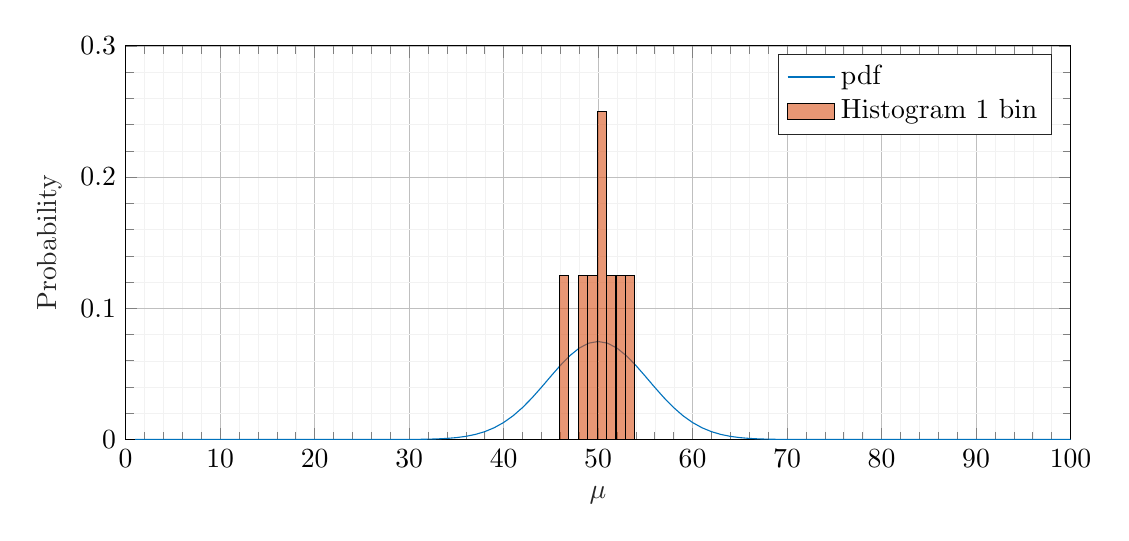
\begin{tikzpicture}

\begin{axis}[%
width=120mm, 
height=50mm, 
at={(5mm,5mm)}, 
scale only axis,
xmin=0,
xmax=100,
xlabel style={font=\color{white!15!black}},
xlabel={$\mu$ \si{\decibel}},
ylabel style={font=\color{white!15!black}},
ylabel={Probability},
ymin=0,
ymax=0.3,
axis background/.style={fill=white},
grid=both,
grid style={line width=.1pt, draw=gray!10},
major grid style={line width=.2pt,draw=gray!50}, 
minor tick num=4,
legend style={legend cell align=left, align=left, draw=white!15!black}
]
\addplot [color=mycolor1]
  table[row sep=crcr]{%
1	3.88753288613558e-20\\
2	2.12976799844824e-19\\
3	1.12657588814019e-18\\
4	5.75385005814751e-18\\
5	2.83743918600713e-17\\
6	1.3510285222346e-16\\
7	6.21115556627748e-16\\
8	2.75708547023195e-15\\
9	1.18167483212333e-14\\
10	4.89007675257209e-14\\
11	1.95390434710717e-13\\
12	7.53808197778718e-13\\
13	2.80794338283003e-12\\
14	1.00991720510473e-11\\
15	3.50714021086796e-11\\
16	1.1759542340013e-10\\
17	3.80712945984117e-10\\
18	1.19007629221712e-09\\
19	3.59188063425429e-09\\
20	1.04674024307622e-08\\
21	2.94527520111863e-08\\
22	8.0017093744719e-08\\
23	2.09898628090369e-07\\
24	5.3162618044904e-07\\
25	1.3000889099313e-06\\
26	3.06979716636403e-06\\
27	6.99868169040538e-06\\
28	1.54061008341285e-05\\
29	3.2744560372424e-05\\
30	6.7197872825729e-05\\
31	0.000133150199239833\\
32	0.000254740530757393\\
33	0.000470569973179873\\
34	0.00083930596077183\\
35	0.00144539429743596\\
36	0.00240337920955625\\
37	0.00385858610996265\\
38	0.00598141625771222\\
39	0.00895261257146183\\
40	0.0129379505820961\\
41	0.0180530721954509\\
42	0.024322414391658\\
43	0.0316396872231062\\
44	0.0397399771717304\\
45	0.0481940005845401\\
46	0.0564323683975447\\
47	0.0638018849939972\\
48	0.0696480041930907\\
49	0.0734097551585918\\
50	0.0747082922100061\\
51	0.0734097551585918\\
52	0.0696480041930907\\
53	0.0638018849939972\\
54	0.0564323683975447\\
55	0.0481940005845401\\
56	0.0397399771717304\\
57	0.0316396872231062\\
58	0.024322414391658\\
59	0.0180530721954509\\
60	0.0129379505820961\\
61	0.00895261257146183\\
62	0.00598141625771222\\
63	0.00385858610996265\\
64	0.00240337920955625\\
65	0.00144539429743596\\
66	0.00083930596077183\\
67	0.000470569973179873\\
68	0.000254740530757393\\
69	0.000133150199239833\\
70	6.7197872825729e-05\\
71	3.2744560372424e-05\\
72	1.54061008341285e-05\\
73	6.99868169040538e-06\\
74	3.06979716636403e-06\\
75	1.3000889099313e-06\\
76	5.3162618044904e-07\\
77	2.09898628090369e-07\\
78	8.0017093744719e-08\\
79	2.94527520111863e-08\\
80	1.04674024307622e-08\\
81	3.59188063425429e-09\\
82	1.19007629221712e-09\\
83	3.80712945984117e-10\\
84	1.1759542340013e-10\\
85	3.50714021086796e-11\\
86	1.00991720510473e-11\\
87	2.80794338283003e-12\\
88	7.53808197778718e-13\\
89	1.95390434710717e-13\\
90	4.89007675257209e-14\\
91	1.18167483212333e-14\\
92	2.75708547023195e-15\\
93	6.21115556627748e-16\\
94	1.3510285222346e-16\\
95	2.83743918600713e-17\\
96	5.75385005814751e-18\\
97	1.12657588814019e-18\\
98	2.12976799844824e-19\\
99	3.88753288613558e-20\\
100	6.85150199158635e-21\\
};

\addplot[ybar interval, fill=mycolor2, fill opacity=0.6, draw=black, area legend] table[row sep=crcr] {%
x	y\\
45.9	0.125\\
46.9	0\\
47.9	0.125\\
48.9	0.125\\
49.9	0.25\\
50.9	0.125\\
51.9	0.125\\
52.9	0.125\\
53.9	0.125\\
};

\addlegendentry{\gls{pdf}}
\addlegendentry{Histogram \SI{1}{\decibel} bin}

\end{axis}
\end{tikzpicture}%
		\caption{The plot shows the Gaussian probability density with the initial data in \autoref{sec:pdf_of_bc}. The histogram is based on the mean data in \autoref{apend:match_field_init}}
		\label{fig:initial_pdf}
\end{figure}

It can be seen in \autoref{fig:initial_pdf} that the measured data, which is plotted in a the histogram, might be a Gaussian distribution if there had been more test subjects. There is no outlaiers and the highest probability lays close to the highest probability of the Gaussian distribution calculated from the data.

mse 1.1835e-04

 \begin{figure}[H]
	\centering
	% This file was created by matlab2tikz.
%
%The latest updates can be retrieved from
%  http://www.mathworks.com/matlabcentral/fileexchange/22022-matlab2tikz-matlab2tikz
%where you can also make suggestions and rate matlab2tikz.
%
%
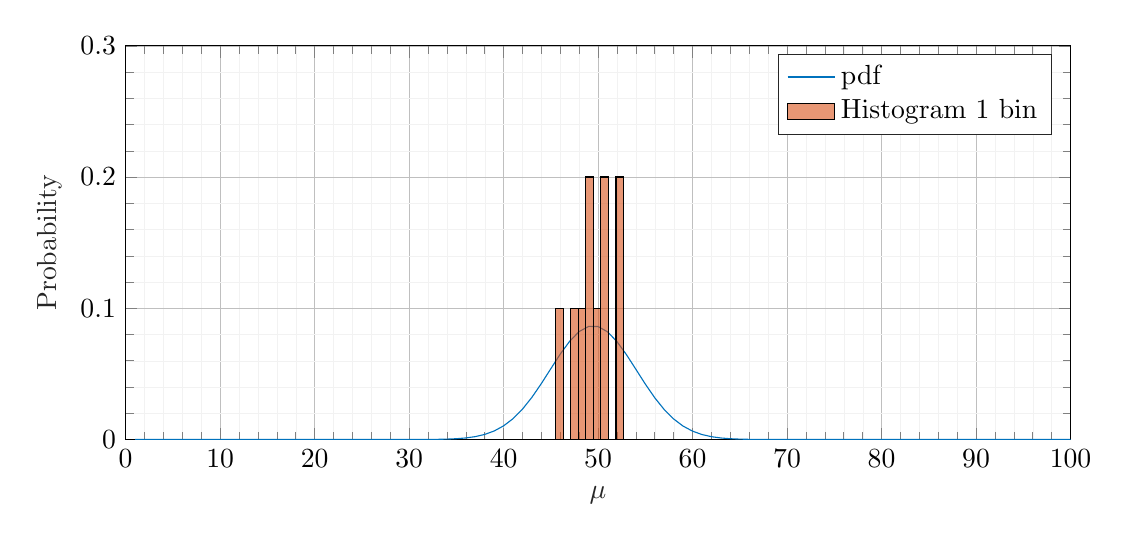
\begin{tikzpicture}

\begin{axis}[%
width=120mm, 
height=50mm, 
at={(5mm,5mm)}, 
scale only axis,
xmin=0,
xmax=100,
xlabel style={font=\color{white!15!black}},
xlabel={$\mu$ \si{\decibel}},
ymin=0,
ymax=0.3,
ylabel style={font=\color{white!15!black}},
ylabel={Probability},
axis background/.style={fill=white},
grid=both,
grid style={line width=.1pt, draw=gray!10},
major grid style={line width=.2pt,draw=gray!50}, 
minor tick num=4,
legend style={legend cell align=left, align=left, draw=white!15!black}
]
\addplot [color=mycolor1]
  table[row sep=crcr]{%
1	7.25124262285027e-26\\
2	6.9736256148195e-25\\
3	6.3975863118078e-24\\
4	5.59867185198651e-23\\
5	4.67374708419392e-22\\
6	3.72183173806484e-21\\
7	2.8272199511126e-20\\
8	2.04867842033147e-19\\
9	1.41611760802938e-18\\
10	9.3376198028466e-18\\
11	5.87332975885434e-17\\
12	3.52406505713514e-16\\
13	2.01704126654263e-15\\
14	1.10127805158289e-14\\
15	5.73575402083945e-14\\
16	2.8496753564529e-13\\
17	1.35055286711742e-12\\
18	6.10575151391139e-12\\
19	2.63316453103856e-11\\
20	1.08324876156756e-10\\
21	4.25098663916887e-10\\
22	1.59133865697685e-09\\
23	5.68259650324332e-09\\
24	1.93571921328358e-08\\
25	6.28997958358421e-08\\
26	1.94969844315782e-07\\
27	5.76496915633775e-07\\
28	1.6260648626584e-06\\
29	4.37512108158142e-06\\
30	1.12293242400631e-05\\
31	2.74934032163068e-05\\
32	6.42117808716936e-05\\
33	0.00014305803734214\\
34	0.000304033293539703\\
35	0.000616369811686115\\
36	0.0011919908169594\\
37	0.00219895222295159\\
38	0.00386963507900279\\
39	0.00649584365155497\\
40	0.0104018946119547\\
41	0.015889150163673\\
42	0.0231526242531135\\
43	0.0321818578233708\\
44	0.042671050443305\\
45	0.0539717985238587\\
46	0.0651196084986405\\
47	0.074949373230504\\
48	0.0822878213165313\\
49	0.0861815809197056\\
50	0.0861003036789081\\
51	0.082055225623091\\
52	0.074596618095108\\
53	0.0646909259841801\\
54	0.053515419063359\\
55	0.0422304615133424\\
56	0.0317895264614316\\
57	0.0228272515066231\\
58	0.0156363190375106\\
59	0.0102170791146777\\
60	0.00636839985272433\\
61	0.00378656333233425\\
62	0.00214768933487952\\
63	0.00116200776455885\\
64	0.000599732982459356\\
65	0.000295269216252836\\
66	0.00013867230774276\\
67	6.21258936366136e-05\\
68	2.6550144473938e-05\\
69	1.08236181584675e-05\\
70	4.20910122803692e-06\\
71	1.56141235907502e-06\\
72	5.52531686266294e-07\\
73	1.865125668e-07\\
74	6.00579277538243e-08\\
75	1.84477719592347e-08\\
76	5.40541240361262e-09\\
77	1.51086298105428e-09\\
78	4.02840068197562e-10\\
79	1.02459345045515e-10\\
80	2.48588952332569e-11\\
81	5.75338460259697e-12\\
82	1.27021232816772e-12\\
83	2.67510340619409e-13\\
84	5.37422889032833e-14\\
85	1.02991901922856e-14\\
86	1.88278760805374e-15\\
87	3.28330265865536e-16\\
88	5.4617502786363e-17\\
89	8.66690616845009e-18\\
90	1.31192100039415e-18\\
91	1.89436040352638e-19\\
92	2.60932914288211e-20\\
93	3.42851817693177e-21\\
94	4.29729711525362e-22\\
95	5.138018237565e-23\\
96	5.86012979396047e-24\\
97	6.37573360669493e-25\\
98	6.61705012857993e-26\\
99	6.55103652169519e-27\\
100	6.18681244638774e-28\\
};

\addplot[ybar interval, fill=mycolor2, fill opacity=0.6, draw=black, area legend] table[row sep=crcr] {%
x	y\\
45.5	0.1\\
46.3	0\\
47.1	0.1\\
47.9	0.1\\
48.7	0.2\\
49.5	0.1\\
50.3	0.2\\
51.1	0\\
51.9	0.2\\
52.7	0.2\\
};

\addlegendentry{\gls{pdf}}
\addlegendentry{Histogram \SI{1}{\decibel} bin}

\end{axis}
\end{tikzpicture}%
		\caption{The plot shows the Gaussian probability density with the initial data in \autoref{sec:pdf_of_bc}. The histogram is based on the mean data in \autoref{apend:matching_in_bier}}
		\label{fig:fam_pdf}
\end{figure}

It can be seen in \autoref{fig:fam_pdf} that the measured data, which is plotted in a the histogram, might be a Gaussian distribution if there had been more test subjects. There is no outlaiers and two the highest probability lays close to the highest probability of the Gaussian distribution calculated from the data, but there is also one histogram bar that have high probability but lays at the high end of the test subject data. 

mse 1.3325e-04

 \begin{figure}[H]
	\centering
	% This file was created by matlab2tikz.
%
%The latest updates can be retrieved from
%  http://www.mathworks.com/matlabcentral/fileexchange/22022-matlab2tikz-matlab2tikz
%where you can also make suggestions and rate matlab2tikz.
%
%
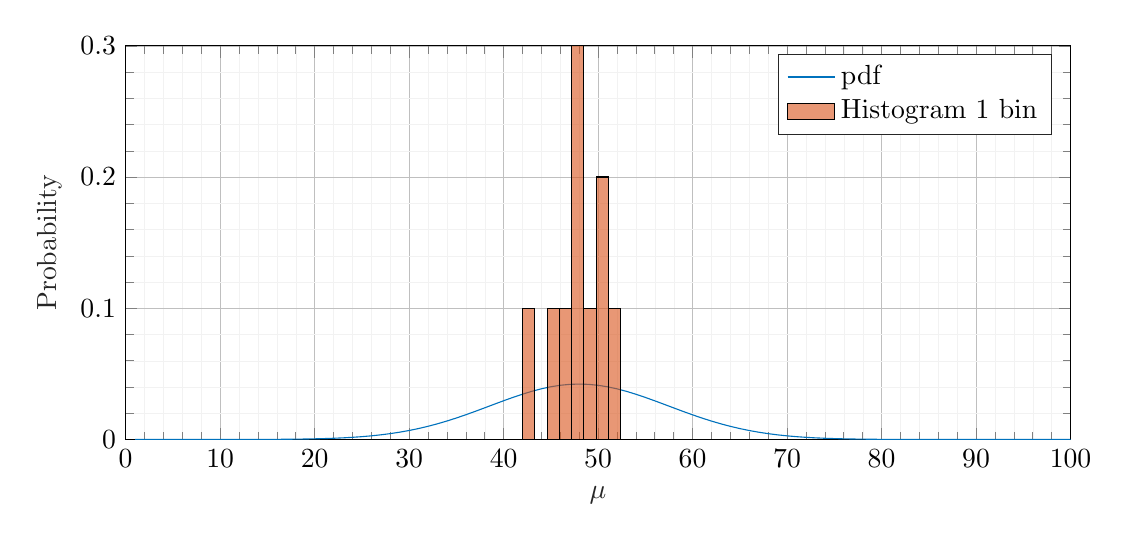
\begin{tikzpicture}

\begin{axis}[%
width=120mm, 
height=50mm, 
at={(5mm,5mm)}, 
scale only axis,
xmin=0,
xmax=100,
xlabel style={font=\color{white!15!black}},
xlabel={$\mu$ \si{\decibel}},
ymin=0,
ymax=0.3,
ylabel style={font=\color{white!15!black}},
ylabel={Probability},
axis background/.style={fill=white},
grid=both,
grid style={line width=.1pt, draw=gray!10},
major grid style={line width=.2pt,draw=gray!50}, 
minor tick num=4,
legend style={legend cell align=left, align=left, draw=white!15!black}
]
\addplot [color=mycolor1]
  table[row sep=crcr]{%
1	1.75976893619116e-07\\
2	2.96499745056968e-07\\
3	4.93991536925927e-07\\
4	8.13844064187308e-07\\
5	1.32583475470207e-06\\
6	2.13581732660697e-06\\
7	3.40224291852152e-06\\
8	5.35911454274503e-06\\
9	8.34732393453135e-06\\
10	1.28566553755954e-05\\
11	1.95810170354727e-05\\
12	2.94896076905044e-05\\
13	4.39166548273957e-05\\
14	6.46719589849264e-05\\
15	9.41736250152641e-05\\
16	0.000135602927916385\\
17	0.000193079138766793\\
18	0.000271849254501927\\
19	0.000378483932135175\\
20	0.000521066622631758\\
21	0.000709358161969407\\
22	0.000954914290311572\\
23	0.00127112927911342\\
24	0.00167317574151511\\
25	0.00217780957859338\\
26	0.0028030106971015\\
27	0.00356743537056704\\
28	0.00448966544515434\\
29	0.00558725320592597\\
30	0.00687557832773972\\
31	0.00836655406580708\\
32	0.010067242198247\\
33	0.0119784581374744\\
34	0.0140934665522146\\
35	0.0163968810479707\\
36	0.0188638863082879\\
37	0.0214598954485423\\
38	0.0241407378815024\\
39	0.0268534436253593\\
40	0.0295376499824088\\
41	0.032127608608523\\
42	0.0345547192081637\\
43	0.0367504654059601\\
44	0.0386495841689526\\
45	0.04019326767272\\
46	0.0413321800173968\\
47	0.0420290735000968\\
48	0.0422608110765178\\
49	0.0420196418628372\\
50	0.0413136316004929\\
51	0.0401662147382492\\
52	0.0386149028265732\\
53	0.0367092485175083\\
54	0.0345082192835356\\
55	0.0320771748484953\\
56	0.0294846638631276\\
57	0.0267992572672885\\
58	0.0240866189405342\\
59	0.0214069814817918\\
60	0.0188131505990801\\
61	0.0163491108319253\\
62	0.0140492535748875\\
63	0.0119382005850894\\
64	0.0100311563447815\\
65	0.00833469351204139\\
66	0.00684785848176511\\
67	0.00556347865475572\\
68	0.00446955805759455\\
69	0.00355066130314675\\
70	0.00278920489270886\\
71	0.00216659679796413\\
72	0.00166418760427849\\
73	0.00126401717780078\\
74	0.000949358354038619\\
75	0.000705072675158925\\
76	0.000517802447663675\\
77	0.000376028551051798\\
78	0.000270025047238332\\
79	0.00019174046994973\\
80	0.000134632537568948\\
81	9.34787255540803e-05\\
82	6.41803441194286e-05\\
83	4.35730346184298e-05\\
84	2.9252304145117e-05\\
85	1.94190893784903e-05\\
86	1.27474743937922e-05\\
87	8.27457969539329e-06\\
88	5.31121944111089e-06\\
89	3.37107996709413e-06\\
90	2.11577933715202e-06\\
91	1.31310119158659e-06\\
92	8.05846876076769e-07\\
93	4.89027593725223e-07\\
94	2.93454457660743e-07\\
95	1.74130386509985e-07\\
96	1.02172712748421e-07\\
97	5.92818559724943e-08\\
98	3.40122346612011e-08\\
99	1.92963447144267e-08\\
100	1.08253373275121e-08\\
};

\addplot[ybar interval, fill=mycolor2, fill opacity=0.6, draw=black, area legend] table[row sep=crcr] {%
x	y\\
42	0.1\\
43.3	0\\
44.6	0.1\\
45.9	0.1\\
47.2	0.3\\
48.5	0.1\\
49.8	0.2\\
51.1	0.1\\
52.4	0.1\\
};

\addlegendentry{\gls{pdf}}
\addlegendentry{Histogram \SI{1}{\decibel} bin}

\end{axis}
\end{tikzpicture}%
		\caption{The plot shows the Gaussian probability density with the initial data in \autoref{sec:pdf_of_bc}. The histogram is based on the mean data in \autoref{apend:matching_in_bier}}
		\label{fig:bier_pdf}
\end{figure}

It can be seen in \autoref{fig:bier_pdf} that the measured data for the \gls{bier} test, which is plotted in a the histogram, have the same tendency as in initial test \autoref{fig:fam_pdf} and the familiarization test \autoref{fig:initial_pdf}. The distribution might be a Gaussian distribution if there had been more test subjects. There is no outlaiers and the highest probability lays close to the highest probability of the Gaussian distribution calculated from the data. 

mes 1.3325e-04

To include more data in the comparison between test subject and the Gaussian distribution, all present subject data is merged to one data file, where the mean and variance is calculated. The following figure \autoref{fig:total_pdf} shows the merged subject data compared with the Gaussian distribution.

 \begin{figure}[H]
	\centering
	% This file was created by matlab2tikz.
%
%The latest updates can be retrieved from
%  http://www.mathworks.com/matlabcentral/fileexchange/22022-matlab2tikz-matlab2tikz
%where you can also make suggestions and rate matlab2tikz.
%
\definecolor{mycolor1}{rgb}{0.00000,0.44700,0.74100}%
\definecolor{mycolor2}{rgb}{0.85000,0.32500,0.09800}%
%
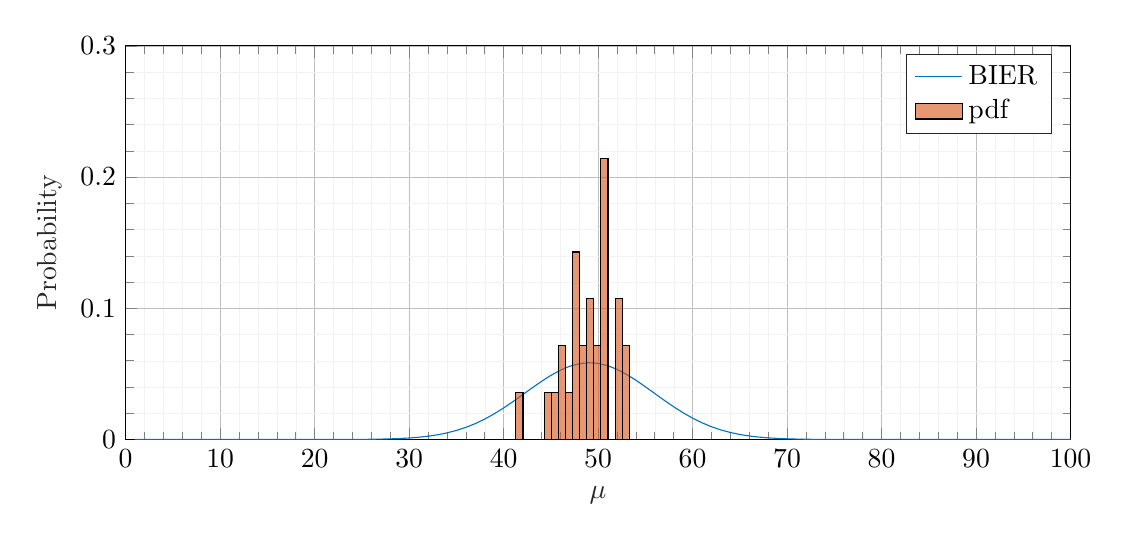
\begin{tikzpicture}

\begin{axis}[%
width=120mm, 
height=50mm, 
at={(5mm,5mm)}, 
scale only axis,
xmin=0,
xmax=100,
xlabel style={font=\color{white!15!black}},
xlabel={$\mu$ \si{\decibel}},
ymin=0,
ymax=0.30,
ylabel style={font=\color{white!15!black}},
ylabel={Probability},
axis background/.style={fill=white},
grid=both,
grid style={line width=.1pt, draw=gray!10},
major grid style={line width=.2pt,draw=gray!50}, 
minor tick num=4,
legend style={legend cell align=left, align=left, draw=white!15!black}
]
\addplot [color=mycolor1]
  table[row sep=crcr]{%
1	9.01034219754882e-13\\
2	2.51009812523995e-12\\
3	6.84371216299437e-12\\
4	1.82618341101851e-11\\
5	4.76923445786109e-11\\
6	1.21900243922119e-10\\
7	3.04938386502976e-10\\
8	7.46571218574015e-10\\
9	1.78888330197399e-09\\
10	4.19512010515232e-09\\
11	9.62849501156914e-09\\
12	2.16283825351717e-08\\
13	4.75489900114573e-08\\
14	1.02308136121882e-07\\
15	2.15442148078078e-07\\
16	4.44020263631701e-07\\
17	8.95625668557875e-07\\
18	1.76807993391386e-06\\
19	3.41608666887847e-06\\
20	6.45962769117923e-06\\
21	1.19546734198352e-05\\
22	2.16530743513101e-05\\
23	3.83842482705996e-05\\
24	6.65944649561856e-05\\
25	0.000113077148999278\\
26	0.000187915752794269\\
27	0.000305635043364694\\
28	0.000486513313743516\\
29	0.000757945419875085\\
30	0.00115566712237925\\
31	0.00172456356014809\\
32	0.00251870482513029\\
33	0.00360020279614776\\
34	0.00503649349545217\\
35	0.00689574529471229\\
36	0.00924029354194626\\
37	0.0121183068715824\\
38	0.0155542740229358\\
39	0.0195393074874385\\
40	0.0240226111137723\\
41	0.0289056590741951\\
42	0.0340405966182711\\
43	0.0392340437594224\\
44	0.0442568605243411\\
45	0.048859582925442\\
46	0.0527922934980413\\
47	0.0558268245874159\\
48	0.0577785906263479\\
49	0.0585251565242688\\
50	0.0580189474172002\\
51	0.0562922657201139\\
52	0.0534538799965585\\
53	0.0496776863857804\\
54	0.0451850857088073\\
55	0.0402235577610565\\
56	0.0350443067991965\\
57	0.0298817541406269\\
58	0.0249371216785499\\
59	0.0203675214538613\\
60	0.0162810219686386\\
61	0.0127372819976759\\
62	0.00975266906177582\\
63	0.00730839198816506\\
64	0.00536008652082168\\
65	0.00384745358218745\\
66	0.00270287897336577\\
67	0.00185836677537929\\
68	0.0012505120668009\\
69	0.000823561361788729\\
70	0.000530830246877145\\
71	0.00033486285914331\\
72	0.000206742575759036\\
73	0.00012492359862392\\
74	7.38772416156205e-05\\
75	4.27590924467894e-05\\
76	2.4221325601087e-05\\
77	1.34282357931694e-05\\
78	7.28604134400339e-06\\
79	3.86915319722988e-06\\
80	2.01090633378741e-06\\
81	1.02286750074447e-06\\
82	5.09211894985224e-07\\
83	2.48101461039605e-07\\
84	1.18307349664425e-07\\
85	5.5213560092053e-08\\
86	2.52192053490206e-08\\
87	1.12737569318095e-08\\
88	4.93239169477602e-09\\
89	2.11202021396818e-09\\
90	8.85095647245183e-10\\
91	3.6302284939487e-10\\
92	1.45723414699552e-10\\
93	5.72501118305298e-11\\
94	2.20127834432921e-11\\
95	8.28371606945251e-12\\
96	3.05089365792487e-12\\
97	1.09971603446035e-12\\
98	3.87958852761604e-13\\
99	1.33949901095746e-13\\
100	4.52637727767328e-14\\
};
\addlegendentry{BIER}

\addplot[ybar interval, fill=mycolor2, fill opacity=0.6, draw=black, area legend] table[row sep=crcr] {%
x	y\\
41.3	0.0357142857142857\\
42.05	0\\
42.8	0\\
43.55	0\\
44.3	0.0357142857142857\\
45.05	0.0357142857142857\\
45.8	0.0714285714285714\\
46.55	0.0357142857142857\\
47.3	0.142857142857143\\
48.05	0.0714285714285714\\
48.8	0.107142857142857\\
49.55	0.0714285714285714\\
50.3	0.214285714285714\\
51.05	0\\
51.8	0.107142857142857\\
52.55	0.0714285714285714\\
53.3	0.0714285714285714\\
};

\addlegendentry{\gls{pdf}}
\addlegendentry{Histogram \SI{1}{\decibel} bin}
\end{axis}
\end{tikzpicture}%
		\caption{The plot shows the Gaussian probability density with the Total data in \autoref{sec:pdf_of_bc}. The histogram is based on the mean data merge of \autoref{apend:matching_in_bier} and \autoref{apend:match_field_init}}
		\label{fig:total_pdf}
\end{figure}

It can be seen in \autoref{fig:total_pdf} that the measured data for the all subject test together, which is plotted in a the histogram, starts to . The distribution might be a Gaussian distribution if there had been more test subjects. There is no outlaiers and the highest probability lays close to the highest probability of the Gaussian distribution calculated from the data. 

mse 7.7464e-05